\section{為何香港人不集中力量發展經濟,而在認同問題上糾纏?}

香港於九七後的經濟,從總量來說仍有明顯增長。自一九九七年至二零一七年其間,香港的人均產出從二萬七千美元增加至四萬六千美元,十分可觀(同期中國的數據則由不足八百美元增加至近九千美元)。但這些經濟增長在香港社會中談得不多,亦未能疏解近年興起的認同問題;香港人也不會拿來四處炫耀,因為香港人發現了「集中力量發展經濟」的虛無。

\begin{figure}[htbp]
    \centering
    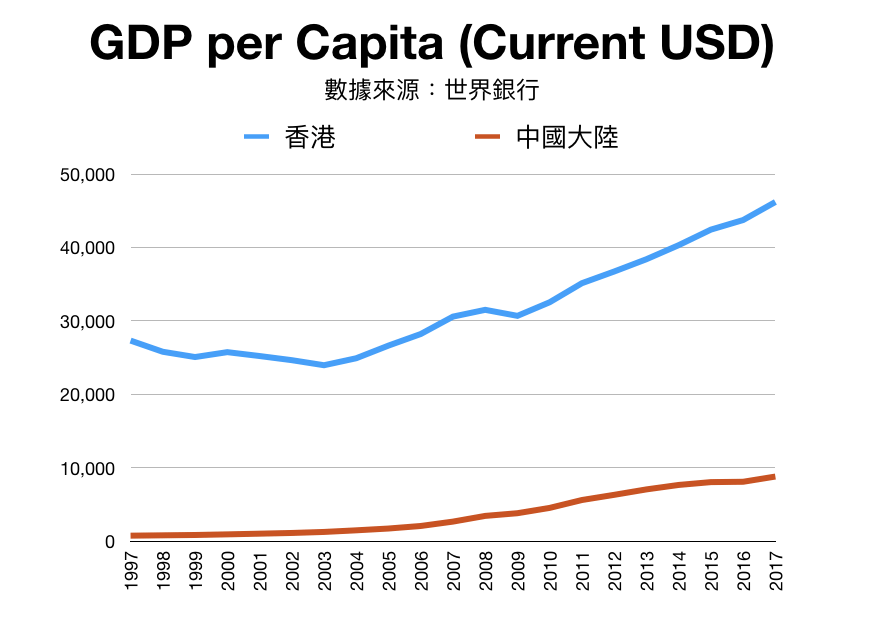
\includegraphics[width=0.7\textwidth]{c09/h-klesson1-009.png}
    \caption{香港經濟近年增長迅速} 
\end{figure}

由於中國大陸和香港在九七後經歷了不同的經濟發展歷程,連帶對經濟發展的社會意義的理解也出現巨大落差。經歷過九七後多年的經濟危機,以及隨之而來的貧富差距擴大和階級流動性減低,社會上特別是年輕人之間不再視經濟發展為首要和唯一的目標,後物質價值的追求變得同樣或更為重要。在這個前提下,集中力量發展經濟的說法變得不再吸引,甚至激發更多人提出認同問題。

這個轉變最開始體現在城市發展和保育當中。回到八、九十年代,主流論述往往會把城市發展等同於社會發展,正如《這是我家》也會把鐵路和高速公路寫入歌詞,視城市建設為自我認同的來源。但到了二零零三年以後的香港,當發展不再是硬道理,越來越多針對城市發展的抗爭出現,強調一系列在抗爭者眼中比城市發展更為重要的價值,甚至認為過急的城市發展有害於營造社會認同。

首個案例是灣仔利東街的重建計劃。市區重建局於二零零四年起展開重建計劃,引發部份居民和商鋪不滿。相對於過去因重建拆遷而起的爭端,利東街的抗爭有三點不同。首先,受影響者強調他們的訴求不在於賠償金額,不是為了要求更多的賠償而做「釘子戶」。第二,他們強調「社區網絡」的意義。利東街又名「喜帖街」,是印刷行業特別是結婚喜帖印刷店聚集的地方,而且商戶之間會互相介紹生意;當地居民也慣於互相幫助,鄰里共生。他們指出無論賠償多少,一旦把他們在空間上打散,便等於毀滅他們賴以為生的人際關係。第三,他們自發提出另類發展方案,既容許作局部重建,同時把街道生活的核心區域保留下來,希望達至雙贏。

\begin{figure}[htbp]
    \centering
    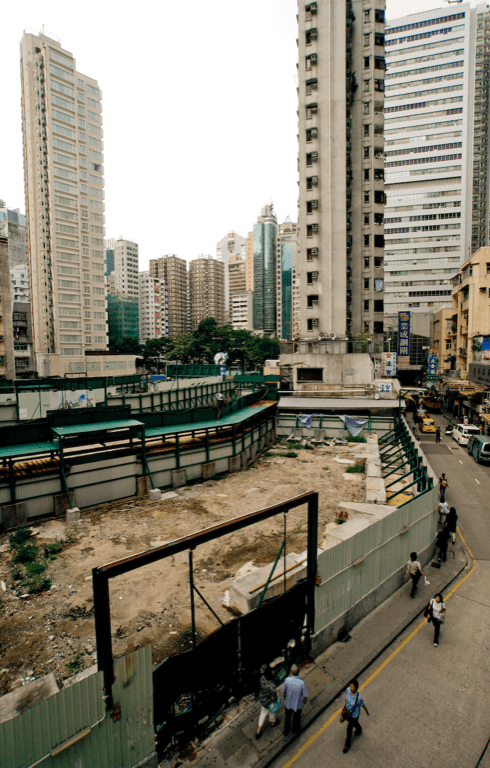
\includegraphics[width=0.7\textwidth]{c09/h-klesson1-011.png}
    \caption{被拆毀後的「喜帖街」} 
\end{figure}

雖然利東街的抗爭失敗告終,原址新建的商場和高尚住宅也於二零一五年開幕,但這次抗爭卻把一些重要的概念帶入主流社會,例如公眾參與和社會影響,以及對地方情感的追求,打破了城市建設在公眾心目中過去一面倒的正面形象。自此之後,又有天星碼頭和皇后碼頭拆卸的抗爭,兩次事件都圍繞與市民生活相關的歷史建築,於是社會中又興起了集體回憶的說法。其中皇后碼頭的抗爭當中,抗爭者自稱為「本土行動」,把城市發展抗爭提升到爭取自主的層次。值得注意的,是這個訴求當時大多被政府和主流媒體所忽視,抗爭往往被定義為年輕人(特別是「八十後」)的發聲嘗試。

\begin{figure}[htbp]
    \centering
    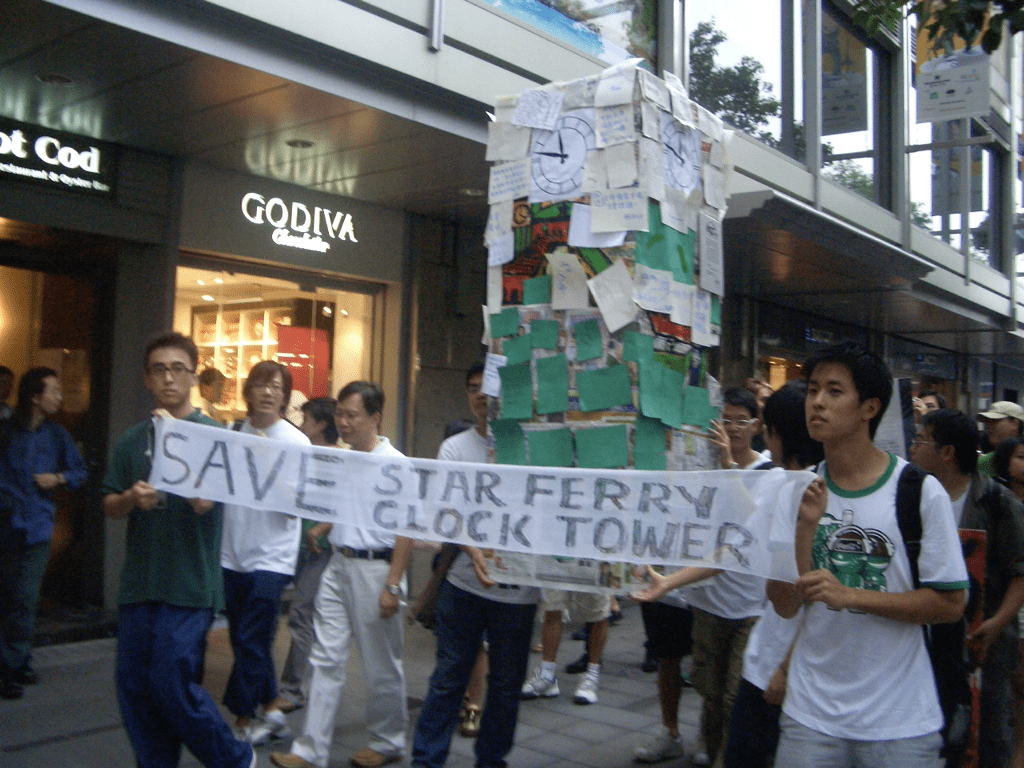
\includegraphics[width=0.7\textwidth]{c09/h-klesson1-012.png}
    \caption{保護天星碼頭運動 2006} 
\end{figure}

不過,不再純粹以經濟建設衡量社會發展的心態,已漸漸在社會中潛移默化。以楊千嬅歌曲《民間傳奇》為例,就借用公主流落民間的故事來借喻後經濟衰退的香港,表明要「告別童話/再造神話」,因為「骨氣煉成花瓣/比霓虹燦爛」,相信「煙花放盡/千金散盡/不減這故事動人」,暗示要在香港過去「發達至上」的法則外尋找另一種的自豪感來源。而以香港情懷為主題的《麥兜》系列電影,也反覆多次以「失落過去的榮耀」為題材,如《麥兜菠蘿油王子》就以王子復國為比喻。到了《麥兜噹噹伴我心》,則更以「風吹雞蛋殻」為主題曲的名字。「風吹雞蛋殻」是廣州話的竭後語,下句是「財散人安樂」,意謂錢財上的損失並不可惜,甚至值得欣慰。

% \begin{figure}[ht!]
%     \centering
%     \includemedia[
%     width=0.6\linewidth,height=0.45\linewidth,
%     activate=pageopen,
%     flashvars={
%         modestbranding=1  % no YT logo in control bar
%         &autohide=1       % controlbar autohide
%         &showinfo=0       % no title and other info before start
%     }
%     ]{}{https://youtu.be/JjWfv_-nLMQ}   % Flash file
%     \caption{《風吹雞蛋殼》 - 麥兜.噹噹伴我心 2012}
% \end{figure}

對於年輕人來說,他們的感受特別明顯。自二零零三年以來香港經濟續步復甦,但年輕人卻分享不到成果,大學畢業生的工資水平幾無增長,樓價卻以倍數上升。對於他們來說,未來的經濟發展是虛幻的,眼前日常生活的品質才是現實的。當政府宣傳的未來經濟發展和他們在乎的日常生活品質有衝突時,他們大多不會相信政府推銷的願景,甚至會選擇對抗。

第一場與中國相關的經濟發展與生活品質的矛盾,在二零零九年的廣深港高速鐵路爭議中出現。高鐵計劃源於二零零零年前後香港政府提出連接廣州和香港的「區域快線」構思,唯粵港兩地因走線和技術選擇一直未達共識,加上香港政府當時忙於處理兩間本地鐵路公司的合併而未有進展。二零零四年起中國大陸大力投資全國高鐵系統,原來的「區域快線」構思也被納入其中,香港政府隨即加速規劃,並在二零零九年末向立法會申請撥款。

對高鐵的質疑,起初來自新界一條名為菜園村的鄉村。由於高鐵計劃在該處設立車廠和救援設施,需要徵地拆遷。田園生活和高速鐵路代表了兩種截然不同的發展觀,兩者在公眾輿論當中構成明顯的對比。而經歷利東街以及天星和皇后碼頭抗爭後,菜園村的抗爭也演化成對另類方案的追求,並聚集了一批專業人士反覆研究政府方案的利弊。他們對政府的方案提出很多質疑,例如預測客量大多數是來往香港和深圳,和政府宣傳的接通全國網絡的說法不乎,而香港本來已有眾多便捷方式來往深圳,高鐵不一定有競爭力。

\begin{figure}[htbp]
    \centering
    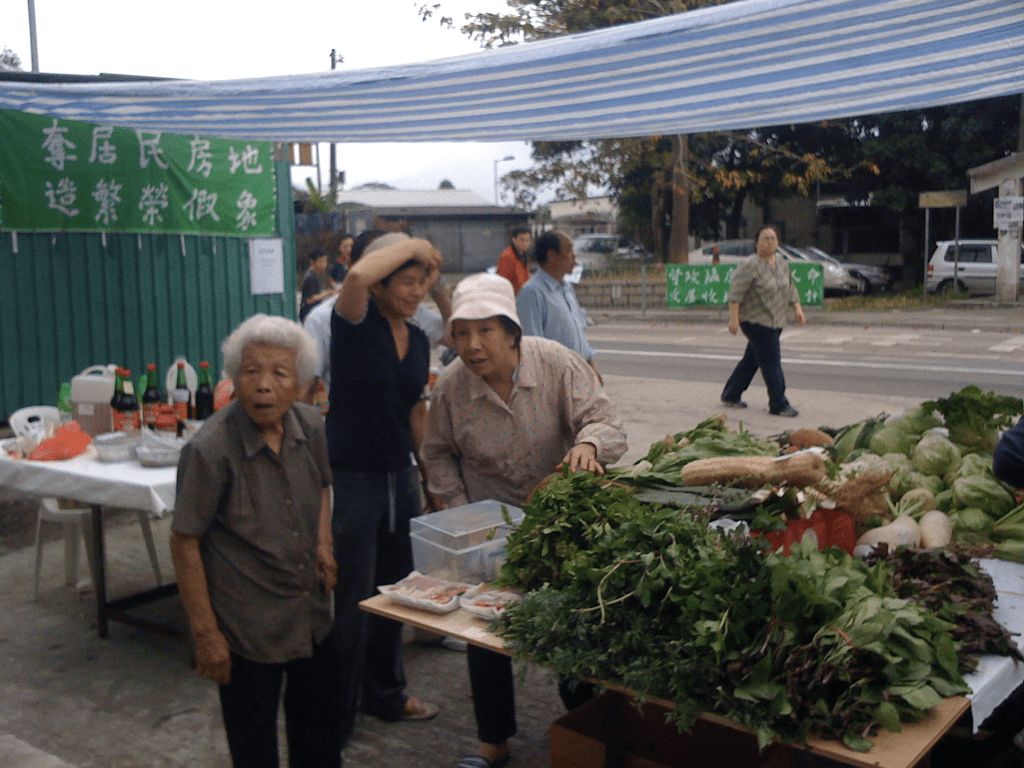
\includegraphics[width=0.7\textwidth]{c09/h-klesson1-010.png}
    \caption{抗爭中的新界石崗菜園村} 
\end{figure}

相對於後來出現的本土思潮,反對中港融合的訴求在反高鐵運動中的角色不算突出,主要的質疑環繞造價、走線和對沿線居民的影響。不過把高鐵爭議放在香港人身分認同的轉變中思考,仍然很有價值,因為在這案例中香港菁英階層的中國想像首次和民間社會出現了明確分歧。

香港政府、親政府輿論和商界對高鐵的支持,一般建基於「邊緣化論」之上。所謂「邊緣化論」是相對於先前八、九十年代「門戶論」的另一種空間想像。在「門戶論」當中,香港是中國大陸和世界之間的中介人,發揮連接和促進交流的角色。然而隨著中國大陸的改革開放走到新的階段,來自世界的企業已開始跳過香港直接走進中國大陸,而中國大陸的企業也能直接走到世界各地投資,香港的角色似乎已變得「多餘」,也就是所謂的「邊緣化」。至於「邊緣化論」和高鐵爭議之間的關係,在於支持者認為中國大陸經濟快速發展,香港經濟要得到快速增長就要和中國大陸連結,所以香港和中國大陸之間要興建一條跑得很快的高鐵,而此興建速度本身也要加快不能再被立法會的辯論所延後。嚴格來說,前面那句話當中的四個「快」在邏輯上沒有必然關係,當時也有輿論提出質疑,但政府卻當作是不證自明的道理來推廣。

但和過去數十年來香港的各種主流中國想像不一樣,「邊緣化論」沒有在社會中形成廣泛共識。相對於八、九十年代,當香港社會恐懼中國大陸的時候,是整個社會一同恐懼;當香港社會視中國大陸為金礦時,也是整個社會一同想像「掘金」。但是來到「邊緣化論」,統治階級和社會大眾卻出現明顯分歧,開始有輿論反問香港一直以來賴以生存,值得香港人自豪的地位,甚至說對中國有所貢獻的地方,都在於其邊緣特質。如果邊緣才是香港的比較優勢,面對「邊緣化論」時則不應感到惶恐,而應思考如何把香港的邊緣特質應用到新的環境當中。

這個「如何利用邊緣位置」的討論最後沒有發生,因為統治階級提出「邊緣化論」的目的恐怕不是真的要探討香港的發展定位,而是要向中共表達其忠誠。如前文所述,中共在九十年代開始積極通過中國大陸的發展機會來收編香港本地資本家,讓他們成為其在港政治代理人。高鐵爭議成為他們表達政治忠誠的機會,所以親政府輿論和商界的支持都會環繞於宏大論述,不願進入具體成本效益(如實際列車班次和客量預測)的討論,以求站穩其道德高地。不過,他們這樣做卻產生一個很實在的代價:自高鐵爭議開始,社會輿論出現了對統治階級的潛在懷疑,每當他們提出中港融合可以為香港帶來好處的時候,都會被質疑只是為自己的利益說話。特別是當一般香港人都感受不到那些好處,甚至是先感受到壞處的時候,矛盾就更為明顯。

以近年中國大陸來港旅客是否過多的爭議為例,親政府輿論和商界就常常集中宣傳遊客來港帶來的經濟貢獻,但這種說法不但無法減輕市民的不滿,反而增加更多的矛盾。在許多人的眼中,所謂的經濟貢獻最明顯的體現是購物區的租金增加,得益的是地產商,而一般人卻因為租金上升做成的店舖單一化而受害。按香港中文大學的調查顯示,即使受訪者在回應前被提醒「如果收緊自由行政策,會對本地的零售、旅遊及相關行業造成負面影響」,仍然有高達87.3\%表示仍支持收緊「自由行」政策,可見香港人並非不理解經濟利害所在,而是考慮過後仍然對現況不滿。

歷史建築保育爭議和高鐵爭議,可說是香港社會中後物質價值和經濟發展至上主義的首回爭端。香港政府和統治階級無法再以經濟發展來確立民眾支持,反而引發更多的反彈。而當政府的經濟發展是以中港融合為前設時,隨之而來的認同衝突也就火速抗散。

\rule[-10pt]{15cm}{0.05em}

伸延閱讀:

梁啟智(2012):〈高鐵爭議中的邊緣化和融合想像〉,張少強、梁啟智、陳嘉銘編《香港‧論述.傳媒》,香港:牛津大學出版社。

葉蔭聰(2010):〈當「文物保育」變成活化〉,許寶強編《重寫我城的歷史故事》,香港:牛津大學出版社。